\section{Lattice edits, errors, and feature boundaries}
\label{sec:edits}

The Python interface exposes element misalignment operations and a parser/application path for MAD-X EFIELD records. The error reader recognizes alignment columns and integrated normal/skew multipole columns through the documented order range. It retains other numeric columns so the caller can reject unsupported nonzero fields instead of silently dropping them. The exact field semantics and units need domain review against the relevant MAD-X/PTC contract. [claim:ERR-01]

The aperture readers and error-table readers are Python-side parsers. They should be treated as converters with explicit supported fields, not as complete MAD-X parsers. Their tests are parser checks; side-by-side example scripts are separate workflow evidence. [claim:API-05]

\begin{center}
\begin{tikzpicture}[node distance=8mm and 13mm, box/.style={draw,rounded corners,align=center,text width=38mm,minimum height=10mm}, decision/.style={draw,diamond,align=center,aspect=2,text width=29mm}, arr/.style={-{Stealth},thick}]
\node[box] (tfs) {Read MAD-X EFIELD/TFS rows};
\node[decision,below=of tfs] (supported) {All nonzero fields supported?};
\node[box,below left=of supported] (reject) {Raise error; no partial application};
\node[box,below right=of supported] (resolve) {Resolve element names and fibres};
\node[box,below=of resolve] (apply) {Call exposed PyPTC edit ABI};
\draw[arr] (tfs)--(supported);
\draw[arr] (supported)--node[above left]{no}(reject);
\draw[arr] (supported)--node[above right]{yes}(resolve);
\draw[arr] (resolve)--(apply);
\end{tikzpicture}
\end{center}
This diagram represents the wrapper's guarded error-table path. The named interpretation of individual MAD-X fields remains a separate review item. [claim:ERR-01]

\begin{figure}[ht]
  \centering
  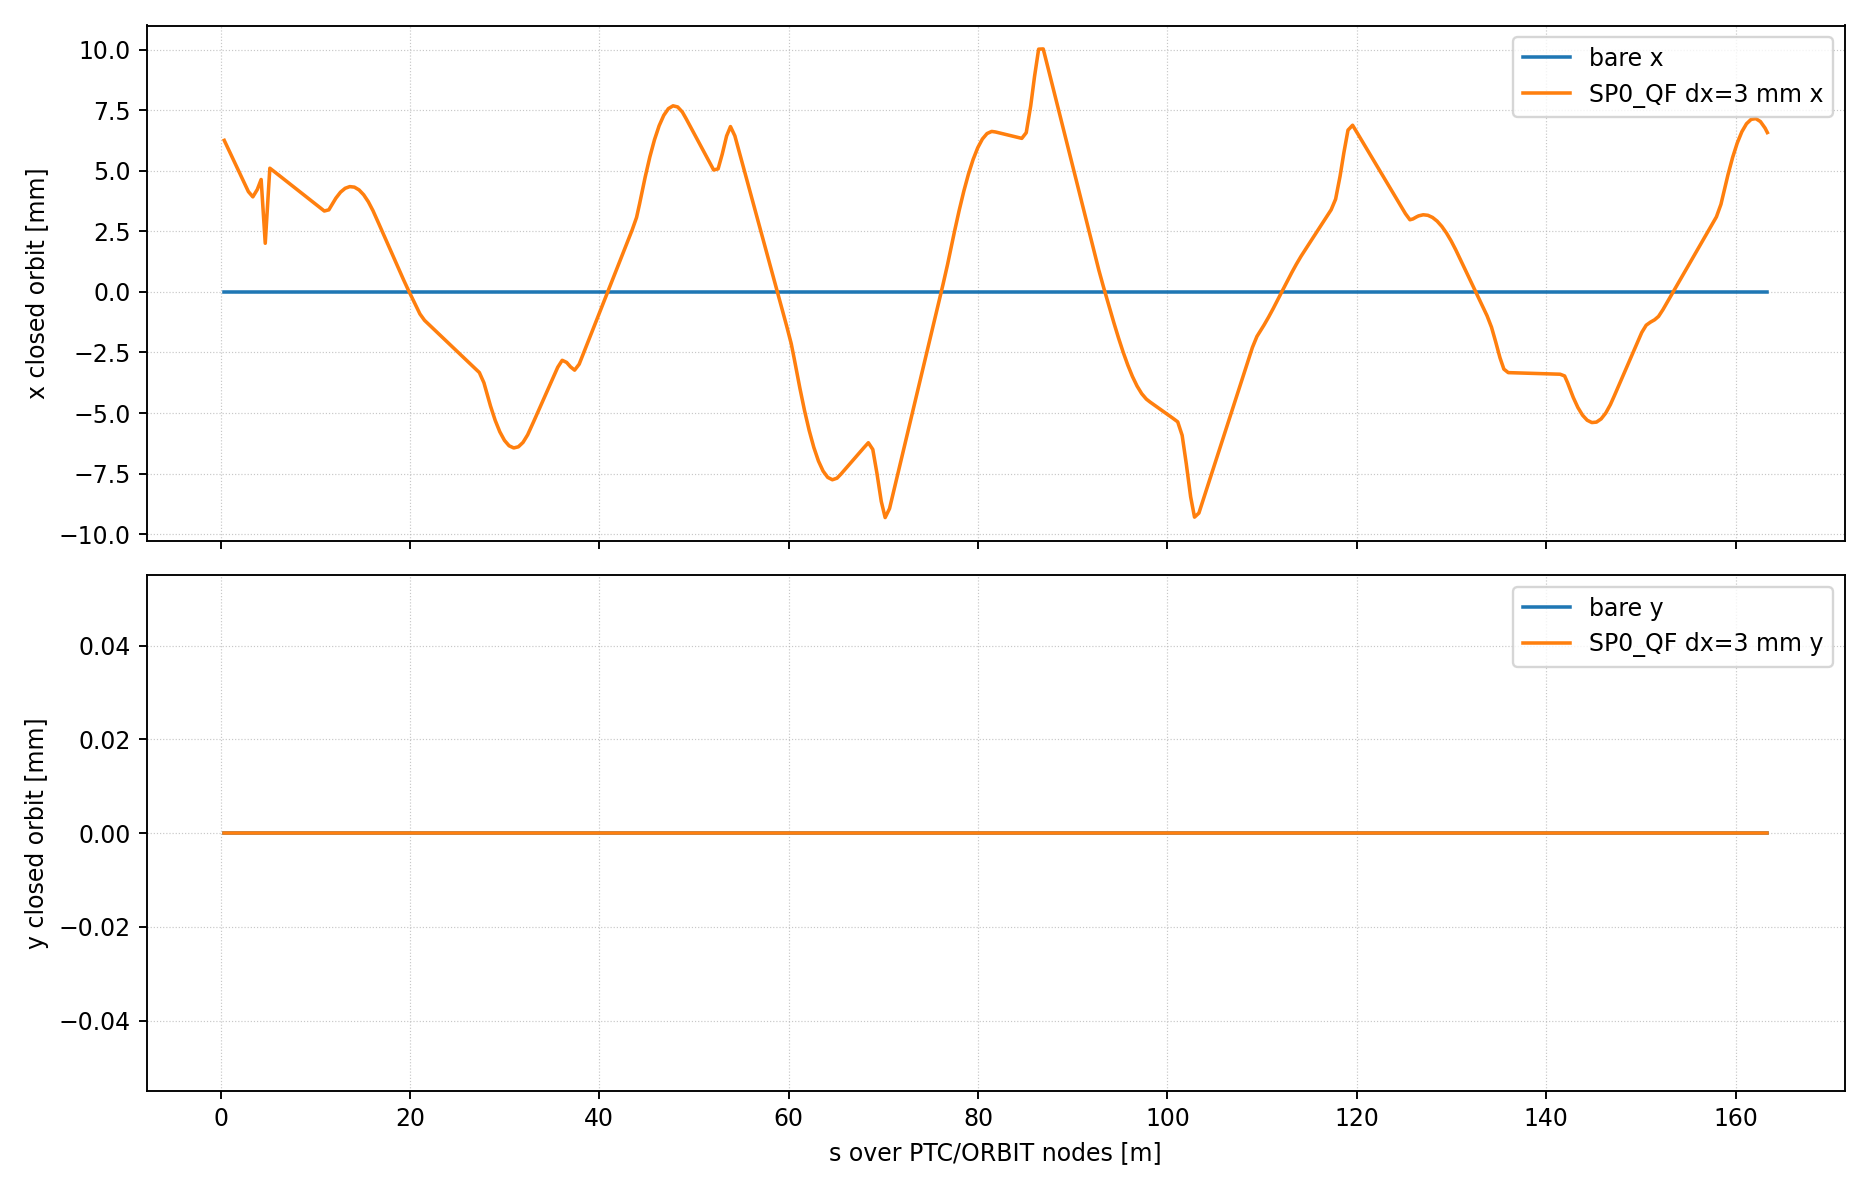
\includegraphics[width=0.84\textwidth]{figures/misalignment_response.png}
  \caption{Single-element misalignment orbit-response plot from the repository example. The example applies a recorded horizontal displacement and compares returned orbit rows. It demonstrates a workflow path, not a machine-calibrated response prediction. [claim:PROV-03] [claim:PROV-04]}
\end{figure}

\begin{figure}[ht]
  \centering
  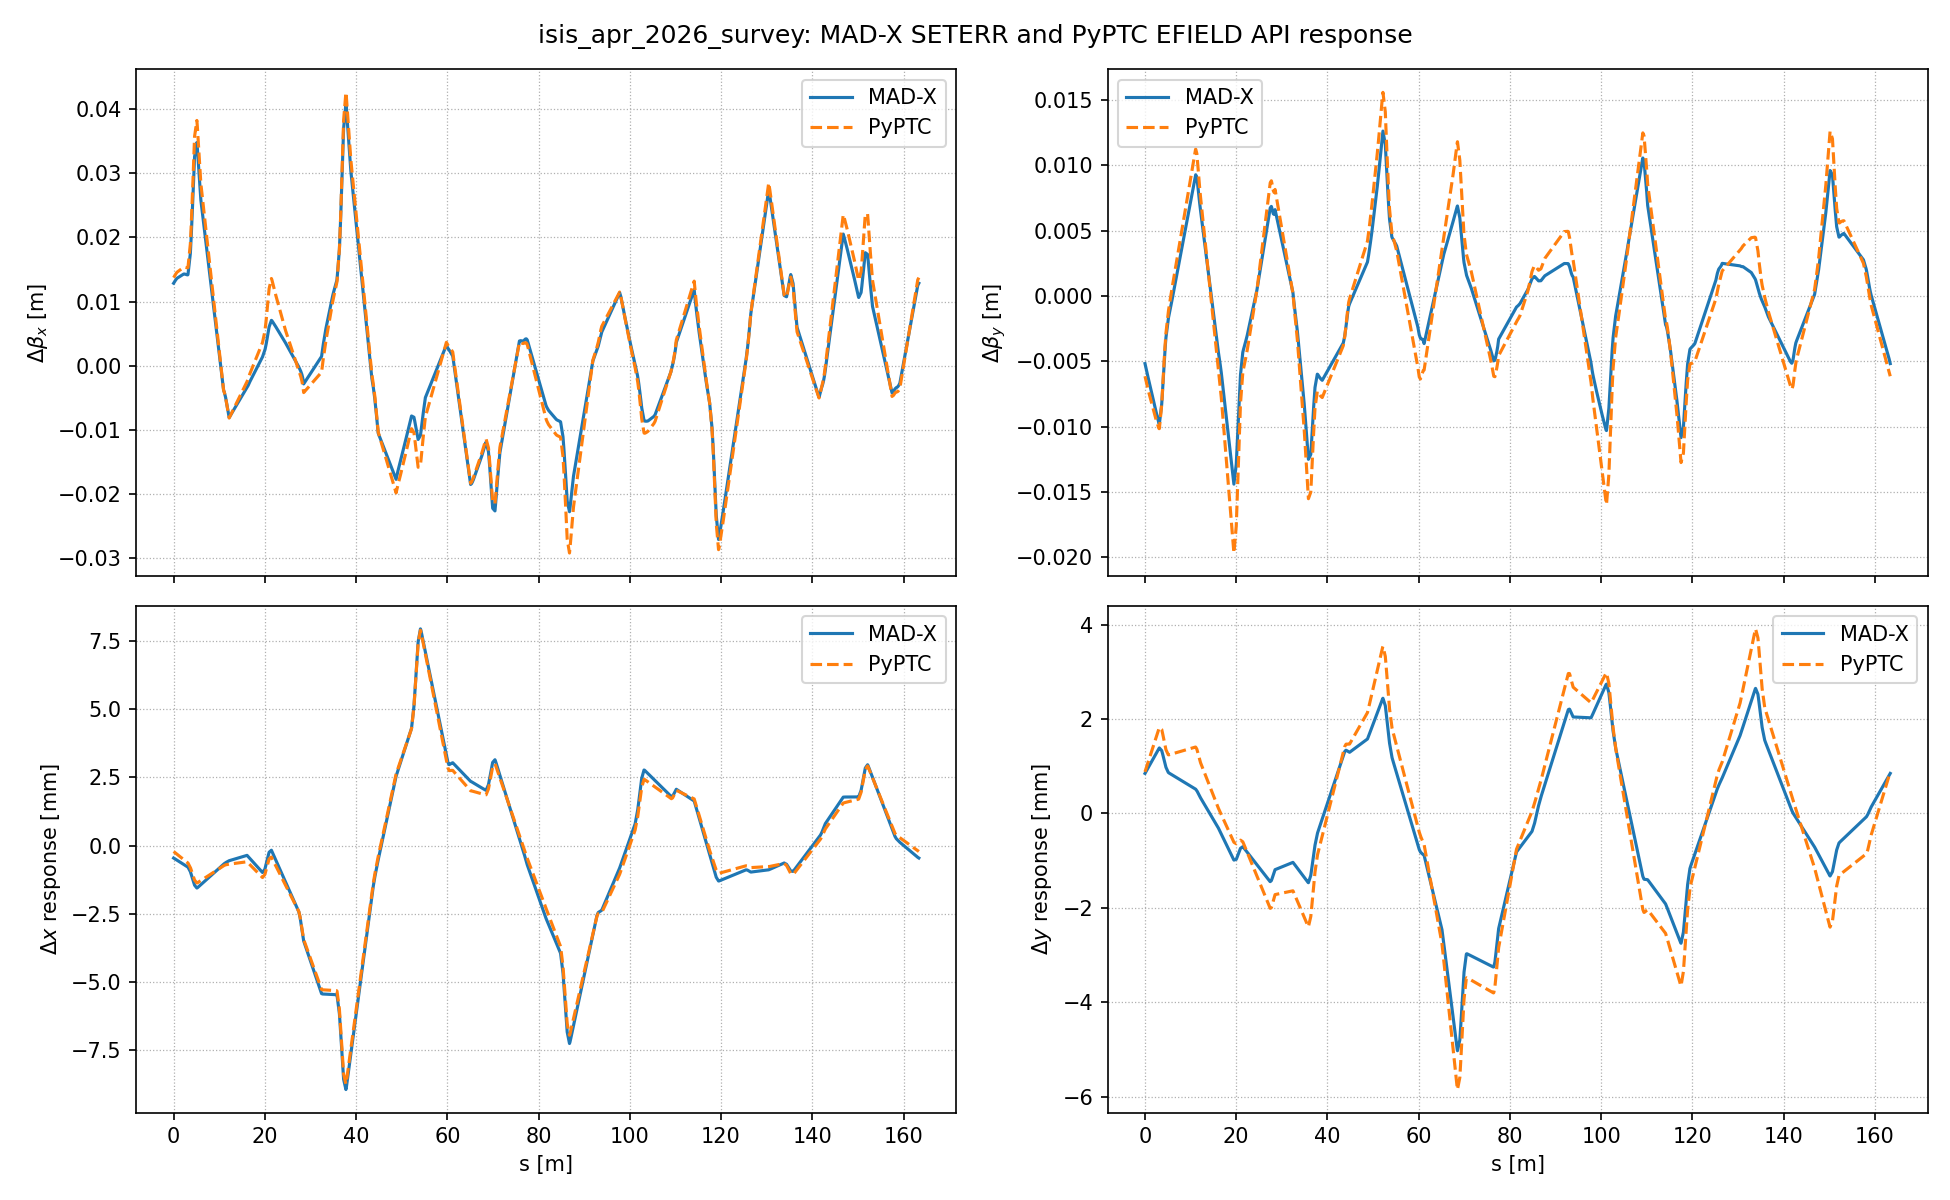
\includegraphics[width=0.88\textwidth]{figures/efield_comparison.png}
  \caption{Stored MAD-X/PyPTC EFIELD side-by-side example for the April 2026 survey table. The companion report records both engines, input and library hashes, and states that the comparison is not tolerance-based acceptance. [claim:PROV-03] [claim:ERR-02] [claim:PROV-04]}
\end{figure}

\begin{figure}[ht]
  \centering
  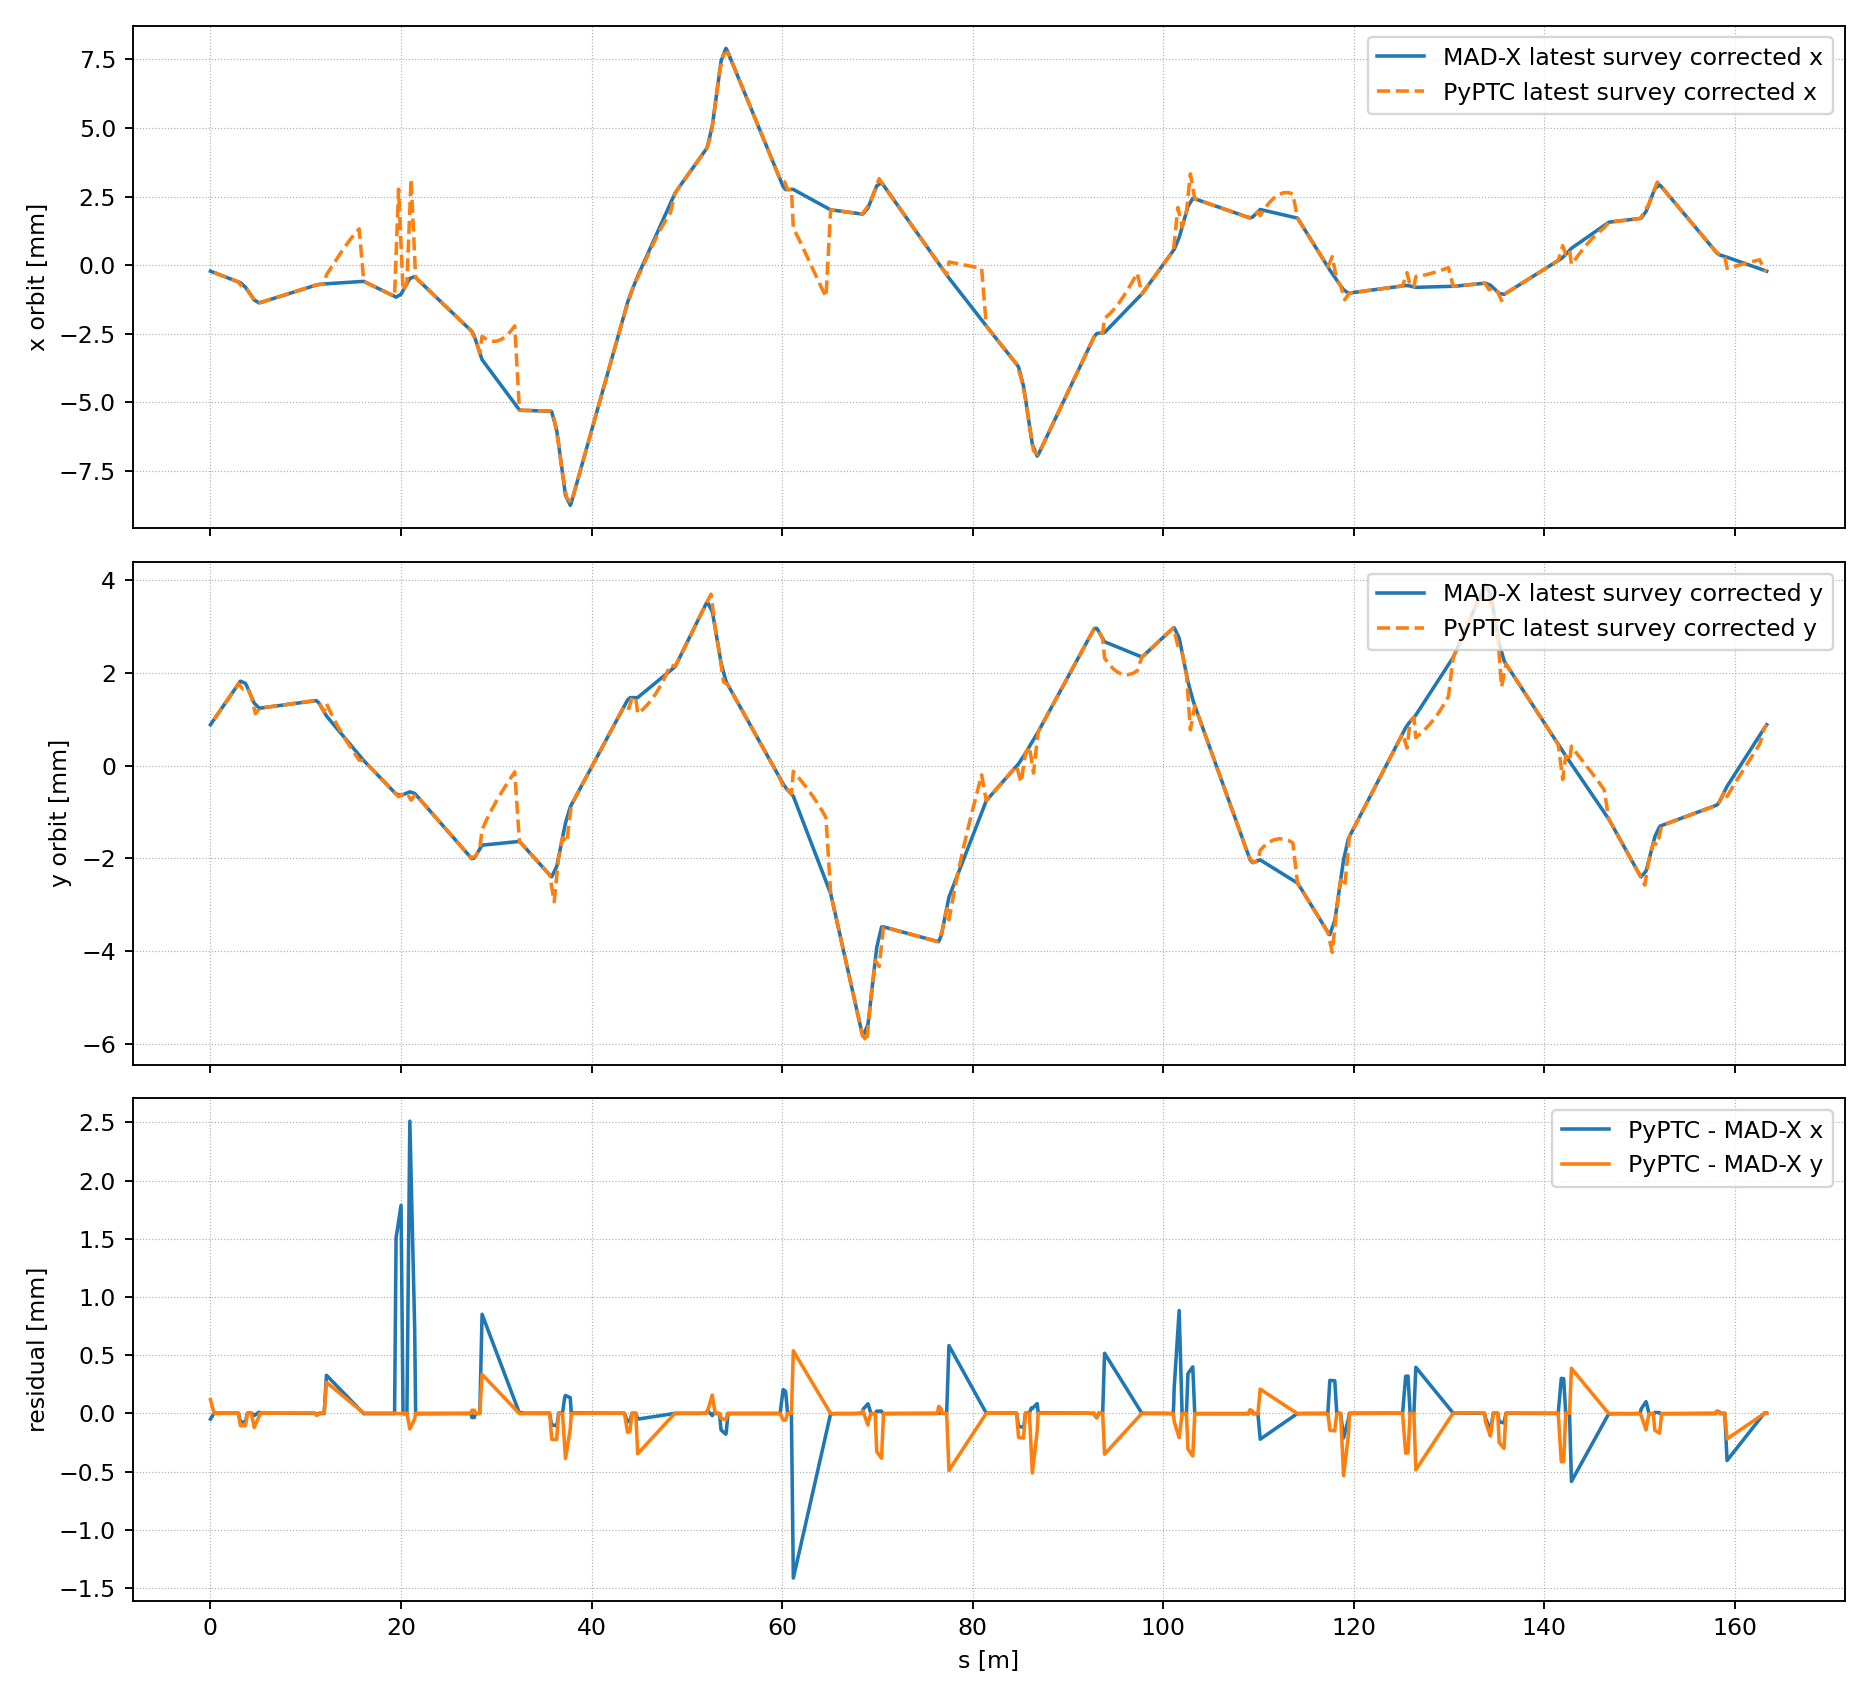
\includegraphics[width=0.88\textwidth]{figures/madx_closed_orbit_comparison.png}
  \caption{Stored full error-table closed-orbit comparison output. This figure belongs to the repository's specific comparison example and its stated table/lattice inputs; it does not define an acceptance tolerance. [claim:PROV-03] [claim:PROV-04]}
\end{figure}

\subsection{Explicitly unexposed paths}

The optics calls \texttt{one\_turn\_map()} and \texttt{normal\_form()} raise a dedicated not-exposed exception. They do not fall back to another calculation. [claim:LIMIT-01]

The normalized-aperture-scan and tune-smear helpers raise the same not-exposed exception. Other PTC features may exist in the underlying library; this guide claims availability only where the repository provides an exposed wrapper path. [claim:LIMIT-02]

\subsection{Examples, tests, and benchmark evidence}

The \texttt{examples/} scripts are runnable demonstrations with user-facing plots and output summaries. \texttt{tests/} contains focused parser and helper checks and separate benchmark-oriented checks. Neither source class should be described as the public API itself. In particular, a MAD-X comparison is evidence for its named case and inputs, not automatic proof of all PyPTC physics behavior. [claim:EXAMPLE-01]
